\paragraph{}This chapter will explain the methodology and requirements for the \ac{SLAM} tuning module, developed for \ac{RUSTLE}. For each implemented tuning technique, a high level overview of its architecture is provided. Test settings, including test algorithms and dataset choices, are also justified.

\begin{figure}[h]
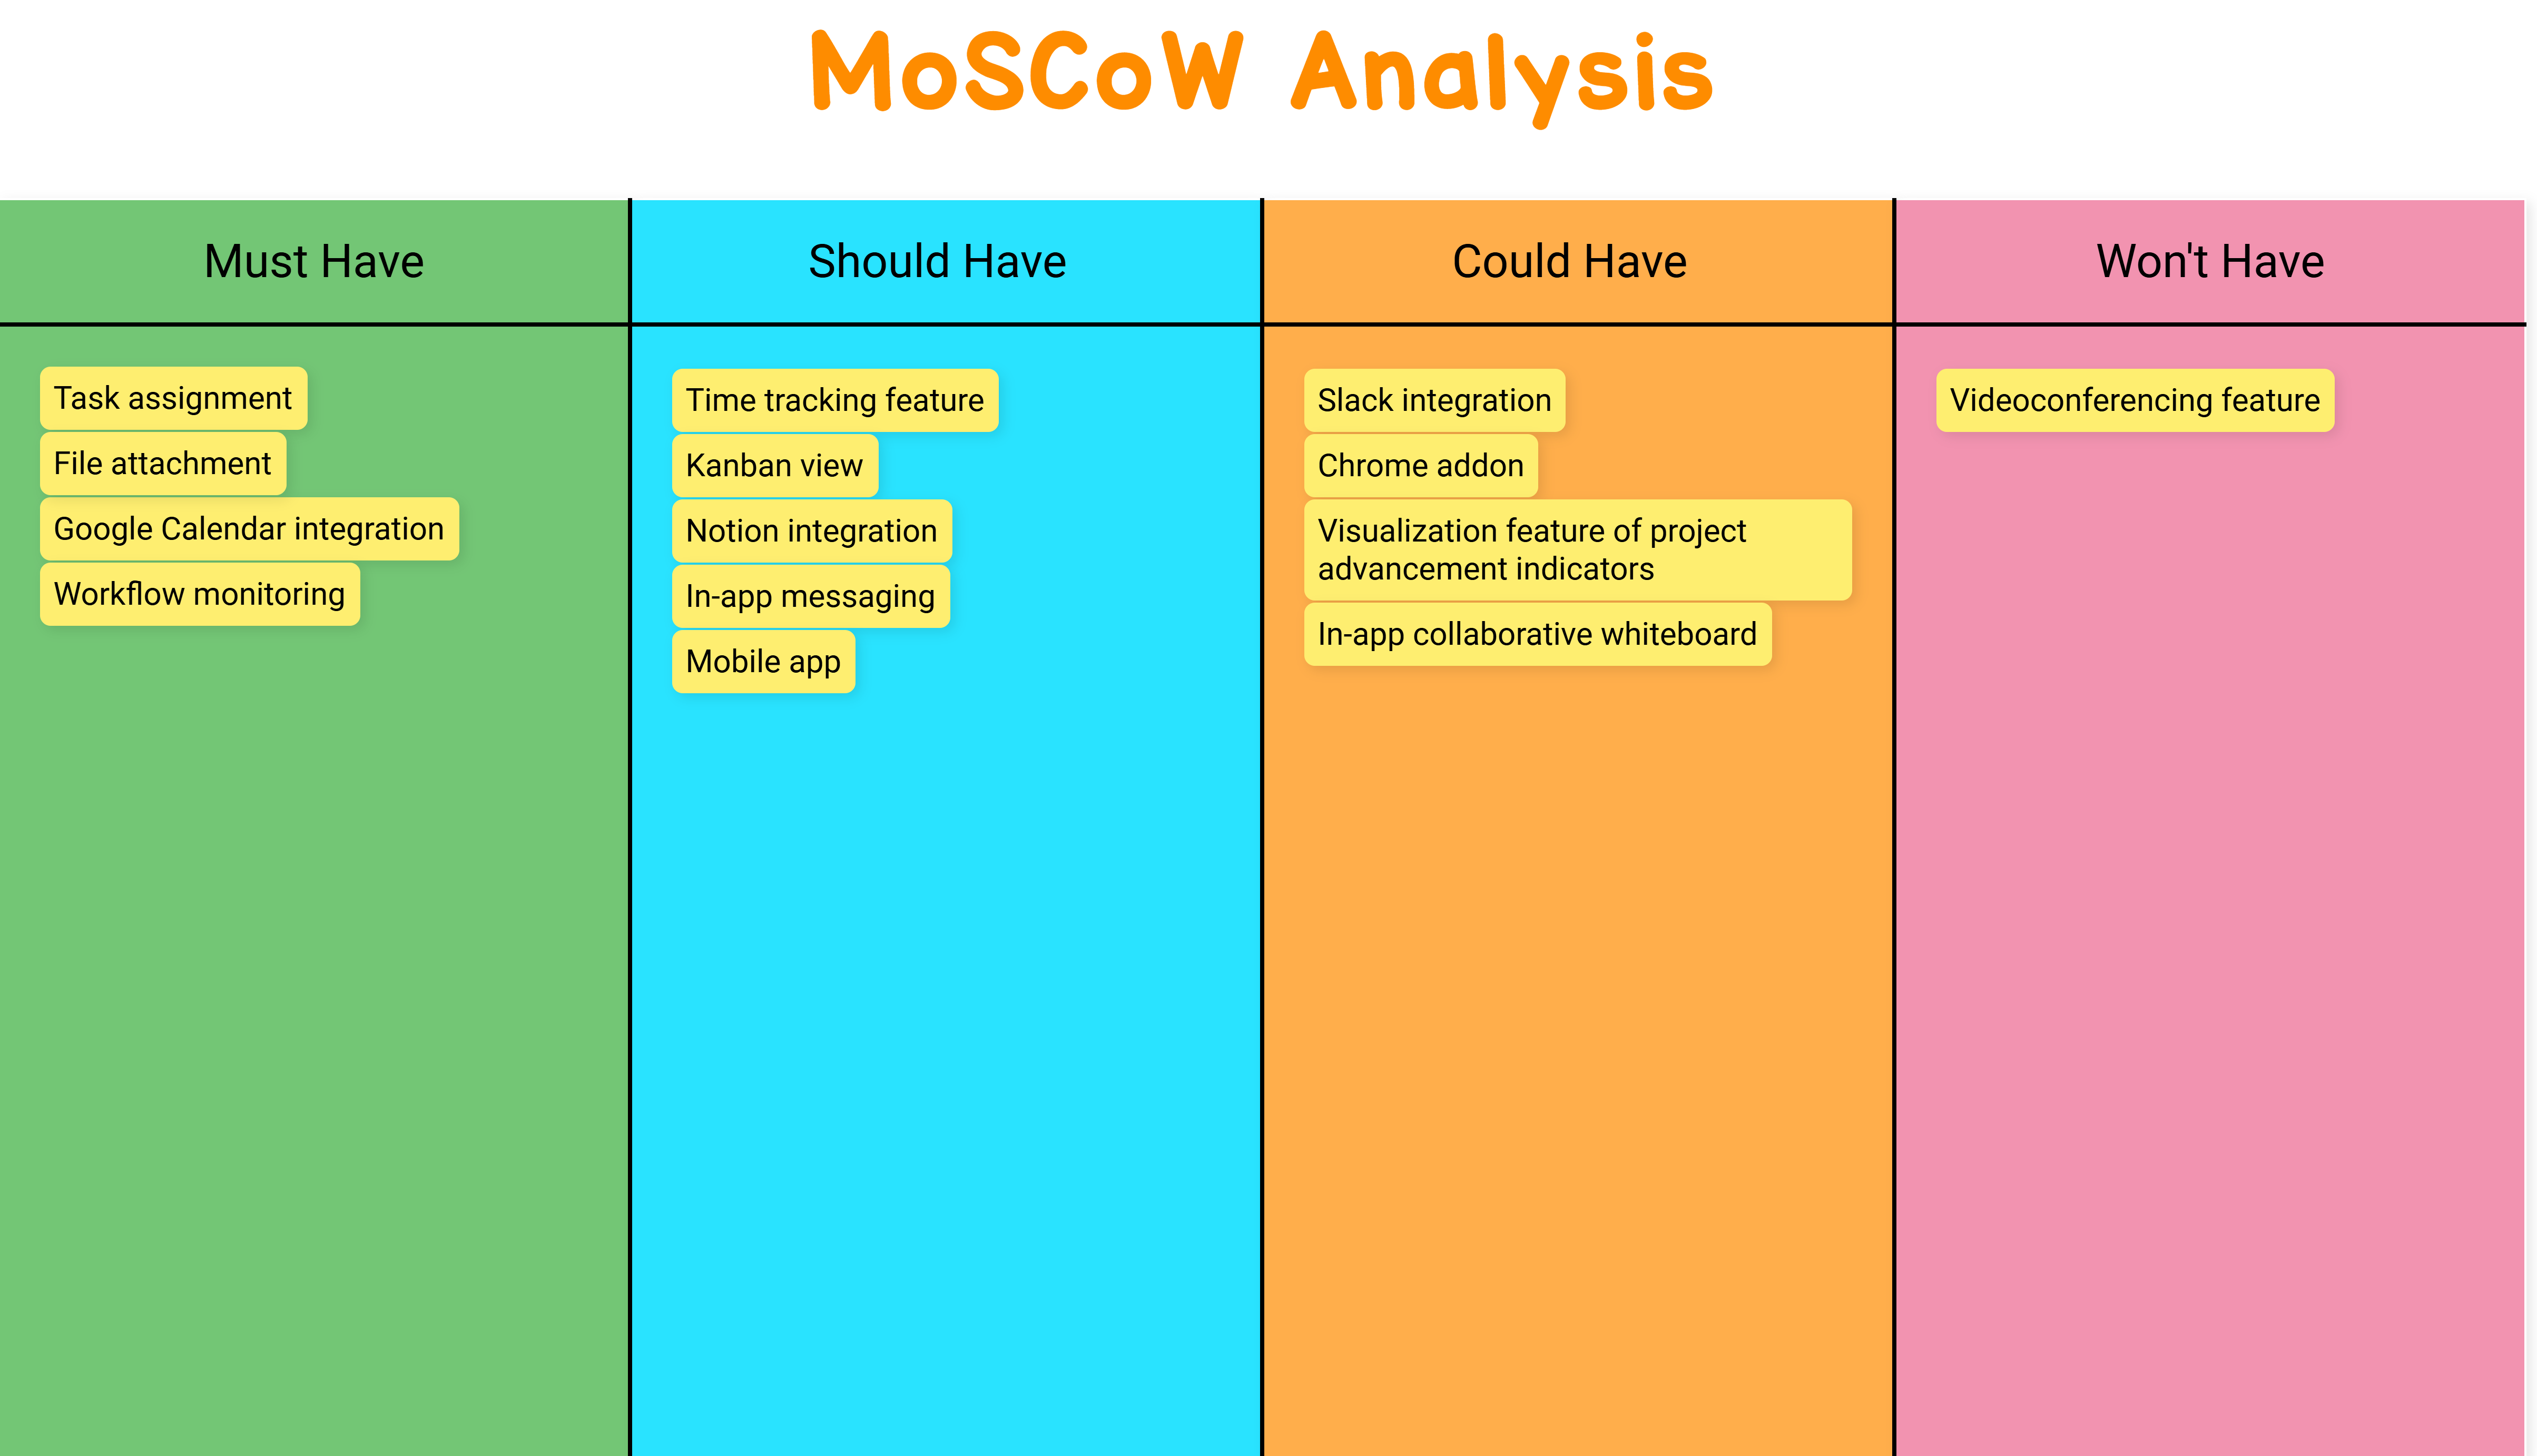
\includegraphics[width=0.85\linewidth]{images/moscow.png}
\end{figure}

\section{\ac{RUSTLE}}

\paragraph{}\ac{RUSTLE} is a command line application, written in Rust, which is designed to simplify the evaluation of SLAM algorithms in mobile robotics.
Its main objective is to provide a simple, stream-lined and reproducible way to run and compare SLAM algorithms. It tracks not only trajectory accuracy(APE or RPE), but also runtime, CPU load and memory usage, offering a more complete assessment of the algorithm's performance.

\paragraph{}At its core, RUSTLE takes three main inputs: a dataset in rosbag format, the SLAM algorithm's parameters in yaml format, and the algorithms themselves as docker images. The reason for using Docker is for reliably reproducing the algorithms across many different platforms and environments.
During execution, the odometry data is streamed into the database(Surrealdb), which, after conclusion, is used to calculate trajectory errors such as the APE and the RPE, using EVO.

\paragraph{}Algorithm executions are run as tests. Each test's configuration is passes as an YAML file, and contains: its name, number of workers, number of iterations, list of algorithms, dataset on which to execute these algorithms and the test type. Additionally, some additional fields might be required, depending on the type of test one wants to execute.



\section{Grid Search}

\section{Random Search}

\section{Simulated Annealing}

\section{Testing}

\subsection{Algorithms}

\subsection{Datasets}